% !TeX spellcheck = en_US
\documentclass[11pt, fleqn, titlepage]{article}
%\usepackage{siunitx}
\usepackage{texfiles/SpeedyGonzales}
\usepackage{texfiles/MediocreMike}
\newcommand{\so}[2]{{#1}\mathrm{e}{#2}}
% \geometry{top=1cm}
\usepackage{hyperref}
\usepackage{amsmath}
\usepackage{ragged2e}
\usepackage{booktabs}
\hypersetup{
	colorlinks=true,
	linkcolor=blue,
	filecolor=magenta,      
	urlcolor=cyan,
}
\usepackage{subfig}
\usepackage{graphicx}
\title{Fairness in Classification}
\author{Oskar Eiler Wiese Christensen s183917 \\ Anders Henriksen s183904}
\date{\today}
	

\pagestyle{plain}
\fancyhf{}
\rfoot{Page \thepage{} of \pageref{LastPage}}

\graphicspath{{Billeder/}}

\begin{document}
	
	\maketitle
	\tableofcontents \newpage
	%\thispagestyle{fancy}
	%\tableofcontents
	\section{Abstract}
	
	
	\section{Introduction}
	
	
	
	\section{Data}
	
	\subsection{Description of Data}
	
	\subsection{Visualization of Data}
	
	\subsection{Bias in Data}
	
	\section{Methods}
	 
	\subsection{Binary Classifier}
	%initialization schemes
	\subsubsection{Feed-forward Neural Network}
	Feed-forward neural networks (FFNN) are the simplest form of a neural network. Information flow in a feed-forward neural is one directional which means that the network has an input layer, and information flow from these nodes through the hidden layers unto the output layer. The main purpose of a FFNN is to approximate a function. In this project $ y = f^*(x) $ maps an input $ \mathbf x $ to a category $ \mathbf y $. The FFNN is thereby a classifier, which goal is to determine the recidvism risk of a person given the input variable $ \mathbf x $. The input variable $ \mathbf x $ contains :::::. The categories of $ \mathbf y $ is either 0 or 1, which corresponds to the classifier classifying a person as either low or medium/high risk of recidivism. Hence, this is a binary classifier which constructs a mapping $ \mathbf y = f(\mathbf x \ ; \mathbf w) $. The goal is to learn the weights that most efficiently approximate the function $ f^* $ through supervised learning. The binary classifier in this project has an input layer, three hidden layers and an output layer. 
	
	\begin{figure}[H]
		\centering
		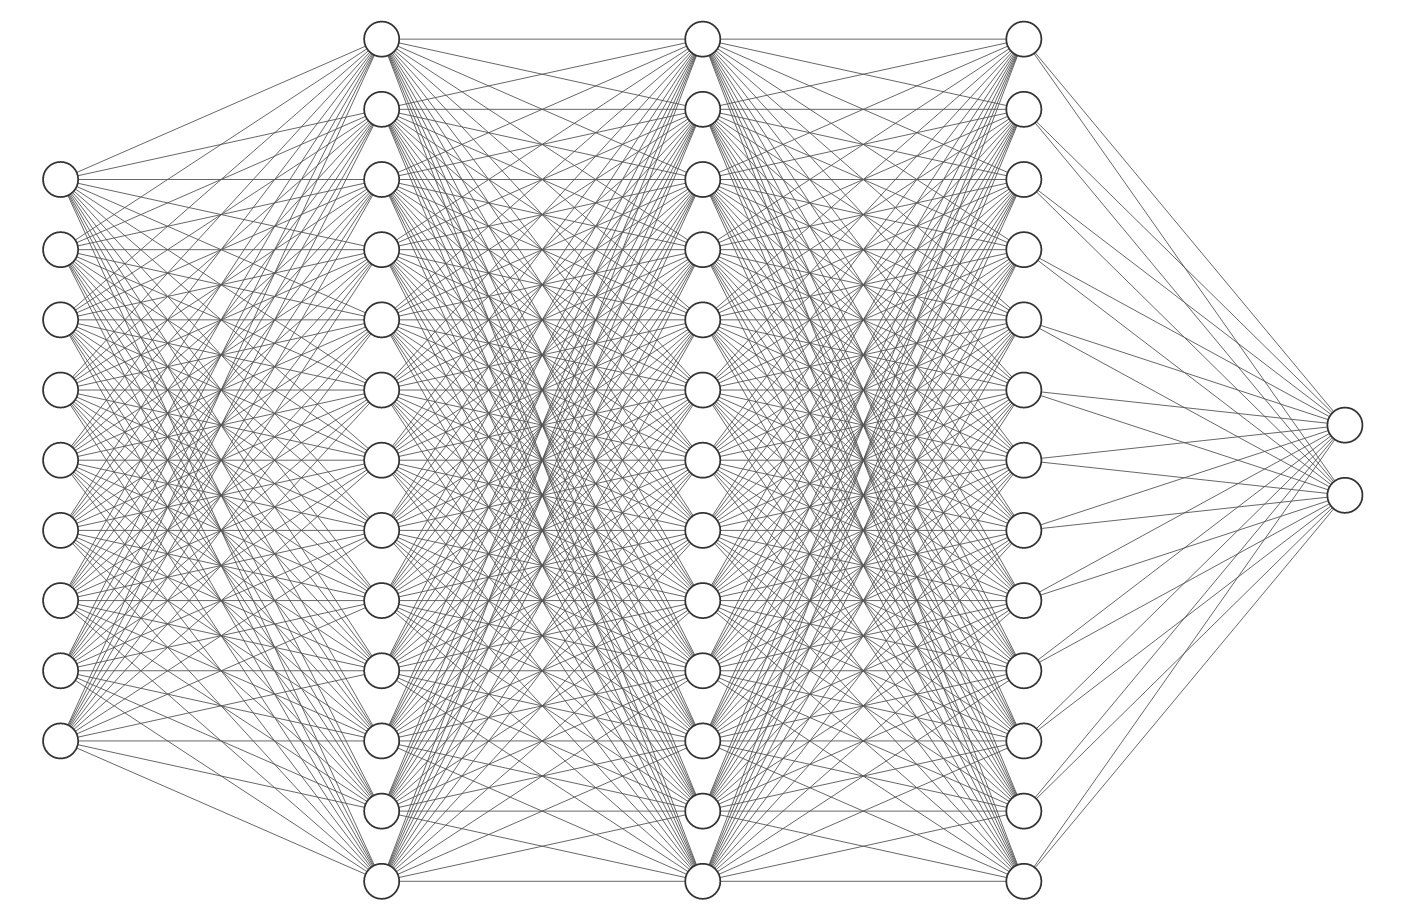
\includegraphics[width=0.5\linewidth]{imgs/ffnn}
		\caption{Visualization of the binary classifier model}
		\label{fig:ffnn}
	\end{figure}
	
	
	\subsubsection{Bayesian Optimization}
	%Bayesian Optimization
	
	To optimize the performance of a neural network an excellent architecture as well as hyperparameters needs to be selected. However, the search for these parameters are usually a costly process of uncertainty balancing exploration of parameters and the exploitation of results. Often the process of finding the optimal parameters and network architecture comes from expert knowledge, biased heuristics or exhaustive sampling from the parameter space. To determine the architecture and hyperparameters of the binary classifier Bayesian Optimization is used. 
	\subparagraph*{Objective Function}
	The objective function that is being optimized in this project is the binary classifier presented above. The fully connected layers are trained on the COMPASS data-set and the accuracy of the model is what BO is trying to optimize. The accuracy of the constructed model is evaluated using non-parametric Gaussian Process (GP) as a function fo the following hyperparameters and 
	\begin{itemize}
		\item Number of units in the first hidden layer \(\in [1, 5000]\) 
		\item Number of units in the second hidden layer \(\in [1, 5000]\) 
		\item Number of units in the third hidden layer \(\in [1, 5000]\)
		\item Dropout probability \(\in [0,1]\)
		\item Activation function \{tanh, ReLU, ReLU6, Sigmoid\}
	\end{itemize}
	The hyperparameters that are not changed are the learning rate, which is set at $ \alpha = 0.001 $. The reason why this parameter is not changed is due to the fact, that the optimizer implemented in this project, is Adaptive Moment Estimation (Adam). Adam is a well known optimizer in the literature and has adaptive learning rate as well as step size. Which is why this learning rate is not an interchangeable hyperparameter. 
	
	
	\subsection{Permutation test}
	
	\subsection{Bias Correction Methods}
	
	\section{Results}
	
	
	\section{Discussion}
	
	
	\section{Conclusion}
	
	%\bibliographystyle{IEEEbib}
	%\bibliography{refs}
	
\end{document}
